\begin{frame}[fragile]{Устойчивоcть (persistence)}
Отличительной особенностью функциональных структур данных является то,
что они всегда \term{устойчивы}{persistent}~--- обновление
функциональной структуры не уничтожает старую версию, а создает
новую, которая с ней сосуществует. \\

Устойчивость достигается путем
\emph{копирования} затронутых узлов структуры данных, и все изменения
проводятся на копии, а не на оригинале. \\

Поскольку узлы никогда
напрямую не модифицируются, все незатронутые узлы могут
\term{совместно использоваться}{be shared} между старой и новой версией структуры
данных без опасения, что изменения одной версии непроизвольно окажутся
видны другой.

\end{frame}

%\chap{Некоторые известные структуры данных в функциональном окружении}

\section{Левоориентированные кучи}
\label{sc:3.1}

\begin{frame}[fragile]{Сигнатура Stack. Реализация через встроенные списки}
\begin{minipage}{.48\textwidth}
\inputminted[firstline=9,lastline=15]{haskell}{code/Stacks.hs}
\end{minipage}
\begin{minipage}{.48\textwidth}
\inputminted{haskell}{code/ListStack.hs}
\end{minipage}
\end{frame}

\begin{frame}[fragile]{Сигнатура Stack. Реализация через новый тип данных}
\begin{minipage}{.48\textwidth}
  \inputminted[firstline=10,lastline=15]{haskell}{code/Stacks.hs}
\end{minipage}
\begin{minipage}{.48\textwidth}
  \inputminted{haskell}{code/CustomStack.hs}
\end{minipage}
\end{frame}

\begin{frame}[fragile]{Конкатенация списков}
\begin{minted}{haskell}
(++) :: STACK l => l a -> l a -> l a
\end{minted}
В императивной среде легко сделать за O(1), если хранить указатель на конец.
\end{frame}

\begin{frame}[fragile]{Конкатенация в императивной среде}
\begin{figure}[h]
%	\centering
	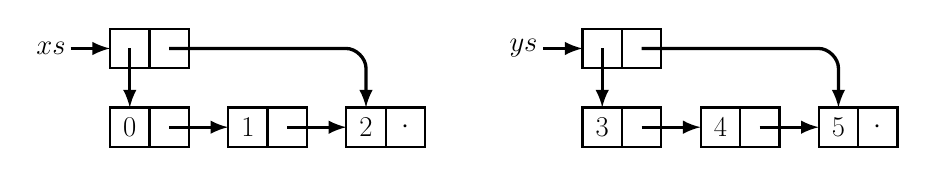
\begin{tikzpicture}[thick,scale=0.5, every node/.style={scale=0.5}]
    \tikzstyle{marrs}=[very thick,-latex]

    \begin{scope}
    
        \foreach \x/\y in {0/0, 0/-2, 3/-2, 6/-2} {
            \draw (\x - 0.5, \y - 0.5) rectangle +(1, 1); \draw (\x + 1 - 0.5, \y - 0.5) rectangle +(1, 1);
        }
        \draw[marrs] (-1.5, 0) -> +(1, 0);
        \draw[marrs] (0, 0) -> +(0, -1.5);
        \draw[marrs] (1, -2) -> +(1.5, 0);
        \draw[marrs] (4, -2) -> +(1.5, 0);
        \draw[marrs] (1, 0) -- (5.5, 0) .. controls (5.75, 0) and (6, -0.25) .. (6, -0.5) -- (6, -1.5);
        
        { \huge
            \draw (-2, 0) node {$xs$};
            \draw (0, -2) node {$0$};
            \draw (3, -2) node {$1$};
            \draw (6, -2) node {$2$};
            \draw (7, -2) node {$\cdot$};
        }
    
    \end{scope}
    
    \begin{scope}[xshift=12cm]
    
        \foreach \x/\y in {0/0, 0/-2, 3/-2, 6/-2} {
            \draw (\x - 0.5, \y - 0.5) rectangle +(1, 1); \draw (\x + 1 - 0.5, \y - 0.5) rectangle +(1, 1);
        }
        \draw[marrs] (-1.5, 0) -> +(1, 0);
        \draw[marrs] (0, 0) -> +(0, -1.5);
        \draw[marrs] (1, -2) -> +(1.5, 0);
        \draw[marrs] (4, -2) -> +(1.5, 0);
        \draw[marrs] (1, 0) -- (5.5, 0) .. controls (5.75, 0) and (6, -0.25) .. (6, -0.5) -- (6, -1.5);
        
        { \huge
            \draw (-2, 0) node {$ys$};
            \draw (0, -2) node {$3$};
            \draw (3, -2) node {$4$};
            \draw (6, -2) node {$5$};
            \draw (7, -2) node {$\cdot$};
        }
    \end{scope}
    
    
    
\end{tikzpicture}\par
	(до)\par
%	\vspace{0.5cm}
	\documentclass[tikz]{standalone}
%\usepackage{fontawesome}

% \newfontfamily{\FA}{Font Awesome 5 Free} % some glyphs missing
\expandafter\def\csname faicon@facebook\endcsname{{\FA\symbol{"F09A}}}
\def\faQuestionSign{{\FA\symbol{"F059}}}
\def\faQuestion{{\FA\symbol{"F128}}}
\def\faExclamation{{\FA\symbol{"F12A}}}
\def\faUploadAlt{{\FA\symbol{"F093}}}
\def\faLemon{{\FA\symbol{"F094}}}
\def\faPhone{{\FA\symbol{"F095}}}
\def\faCheckEmpty{{\FA\symbol{"F096}}}
\def\faBookmarkEmpty{{\FA\symbol{"F097}}}

%\def\faCatt{{\FA\symbol{"F6BE}}}
%\def\faCat{\faicon{cat}}
%\def\faCat{\faicon{yoast}}
\expandafter\def\csname faicon@dog\endcsname{{\FA\symbol{"F4DA}}}
%\def\faDog{\faicon{dog}}
%\def\faDog{{\FA\symbol{"F4DA}}}
%\def\faDogg{{\FA\symbol{"F6D3}}}
%\def\faDogg{{\FA\symbol{"F596}}}

% /usr/share/texlive/texmf-dist/fonts/opentype/public/fontawesome5/FontAwesome5Free-Solid-900.otf
\newfontfamily{\FAS}{FontAwesome5Free-Solid-900.otf}
%\expandafter\def\csname faicon@download\endcsname{{\FAS\symbol{"F6D3}}}
\expandafter\def\csname faicon@cat\endcsname{{\FAS\symbol{"F6BE}}}
\def\faCat{\faicon{cat}}
\expandafter\def\csname faicon@dog\endcsname{{\FAS\symbol{"F6D3}}}
\def\faDog{\faicon{dog}}
\expandafter\def\csname faicon@dragon\endcsname{{\FAS\symbol{"F6D5}}}
\def\faDragon{\faicon{dragon}}
\expandafter\def\csname faicon@fish\endcsname{{\FAS\symbol{"F578}}}
\def\faFish{\faicon{fish}}
\expandafter\def\csname faicon@horse\endcsname{{\FAS\symbol{"F6F0}}}
\def\faHorse{\faicon{horse}}
\expandafter\def\csname faicon@spider\endcsname{{\FAS\symbol{"F717}}}
\def\faSpider{\faicon{spider}}

\expandafter\def\csname faicon@chessking\endcsname{{\FAS\symbol{"F43F}}}
\def\faChessKing{\faicon{chessking}}
\expandafter\def\csname faicon@chessqueen\endcsname{{\FAS\symbol{"F445}}}
\def\faChessQueen{\faicon{chessqueen}}
\expandafter\def\csname faicon@chessrook\endcsname{{\FAS\symbol{"F447}}}
\def\faChessRook{\faicon{chessrook}}
\expandafter\def\csname faicon@chesspawn\endcsname{{\FAS\symbol{"F443}}}
\def\faChessPawn{\faicon{chesspawn}}
\expandafter\def\csname faicon@chessknight\endcsname{{\FAS\symbol{"F441}}}
\def\faChessKnight{\faicon{chessknight}}
\expandafter\def\csname faicon@chessbishop\endcsname{{\FAS\symbol{"F43A}}}
\def\faChessBishop{\faicon{chessbishop}}
\expandafter\def\csname faicon@chess\endcsname{{\FAS\symbol{"F439}}}
\def\faChess{\faicon{chess}}







\usepackage{tikz}
\usetikzlibrary{positioning,trees,decorations.pathreplacing}

\begin{document}
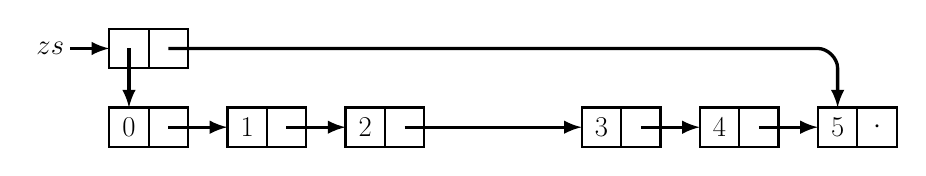
\begin{tikzpicture}[thick,scale=0.5, every node/.style={scale=0.5}]
    \tikzstyle{marrs}=[very thick,-latex]

    
    \begin{scope}
    
        \foreach \x/\y in {0/0, 0/-2, 3/-2, 6/-2} {
            \draw (\x - 0.5, \y - 0.5) rectangle +(1, 1); \draw (\x + 1 - 0.5, \y - 0.5) rectangle +(1, 1);
        }
        \draw[marrs] (-1.5, 0) -> +(1, 0);
        \draw[marrs] (0, 0) -> +(0, -1.5);
        \draw[marrs] (1, -2) -> +(1.5, 0);
        \draw[marrs] (4, -2) -> +(1.5, 0);
        \draw[marrs] (1, 0) -- (17.5, 0) .. controls (17.75, 0) and (18, -0.25) .. (18, -0.5) -- (18, -1.5);
        \draw[marrs] (7, -2) -- +(4.5, 0);
        
        { \huge
            \draw (-2, 0) node {$zs$};
            \draw (0, -2) node {$0$};
            \draw (3, -2) node {$1$};
            \draw (6, -2) node {$2$};
        }
    
    \end{scope}
    
    \begin{scope}[xshift=12cm]
    
        \foreach \x/\y in {0/-2, 3/-2, 6/-2} {
            \draw (\x - 0.5, \y - 0.5) rectangle +(1, 1); \draw (\x + 1 - 0.5, \y - 0.5) rectangle +(1, 1);
        }
        
        \draw[marrs] (1, -2) -> +(1.5, 0);
        \draw[marrs] (4, -2) -> +(1.5, 0);
        
        { \huge
            \draw (0, -2) node {$3$};
            \draw (3, -2) node {$4$};
            \draw (6, -2) node {$5$};
            \draw (7, -2) node {$\cdot$};
        }
    \end{scope}
\end{tikzpicture}
\end{document}
\par
	(после)\par
%	\vspace{0.5cm}
	\caption{Выполнение \texttt{xs concat ys} в императивной среде. Эта операция уничтожает списки-аргументы \texttt{xs} и \texttt{ys} (их использовать больше нельзя)}
	\label{fig:2.4}
\end{figure}
\end{frame}


\begin{frame}[fragile]{Конкатенация в функциональной среде}
В функциональной среде мы не можем деструктивно модифицировать. Поэтому
\begin{itemize}
\item добавляем последний элемент первого списка ко второму
\item добавляем \emph{пред}последний элемент первого списка к резульату
\item и т.д.
\end{itemize}

\inputminted[firstline=50,lastline=54] {haskell}{code/Stacks.hs}
Если нам доступно внутреннее представление, то можно написать более короткий идиоматичный код
\inputminted[firstline=57,lastline=58,gobble=2] {haskell}{code/Stacks.hs}
\end{frame}

%\begin{frame}[fragile]{}
%\inputminted[firstline=50,lastline=54] {haskell}{code/Stacks.hs}
%Если нам доступно внутреннее представление, то можно написать более короткий идиоматичный код
%\inputminted[firstline=57,lastline=58,gobble=2] {haskell}{code/Stacks.hs}
%\end{frame}

\begin{frame}[fragile]{Конкатенация}
\begin{figure}[h]
	\centering
	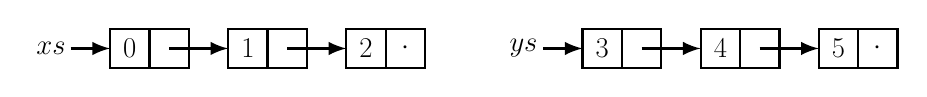
\begin{tikzpicture}[thick,scale=0.5, every node/.style={scale=0.5}]
    \tikzstyle{marrs}=[very thick,-latex]

    \begin{scope}
    
        \foreach \x/\y in {0/0, 3/0, 6/0} {
            \draw (\x - 0.5, \y - 0.5) rectangle +(1, 1); \draw (\x + 1 - 0.5, \y - 0.5) rectangle +(1, 1);
        }
        \draw[marrs] (-1.5, 0) -> +(1, 0);
        \draw[marrs] (1, 0) -> +(1.5, 0);
        \draw[marrs] (4, 0) -> +(1.5, 0);
        
        { \huge
            \draw (-2, 0) node {$xs$};
            \draw (0, 0) node {$0$};
            \draw (3, 0) node {$1$};
            \draw (6, 0) node {$2$};
            \draw (7, 0) node {$\cdot$};
        }
    
    \end{scope}
    
    \begin{scope}[xshift=12cm]
    
        \foreach \x/\y in {0/0, 3/0, 6/0} {
            \draw (\x - 0.5, \y - 0.5) rectangle +(1, 1); \draw (\x + 1 - 0.5, \y - 0.5) rectangle +(1, 1);
        }
        \draw[marrs] (-1.5, 0) -> +(1, 0);
        \draw[marrs] (1, 0) -> +(1.5, 0);
        \draw[marrs] (4, 0) -> +(1.5, 0);
        
        { \huge
            \draw (-2, 0) node {$ys$};
            \draw (0, 0) node {$3$};
            \draw (3, 0) node {$4$};
            \draw (6, 0) node {$5$};
            \draw (7, 0) node {$\cdot$};
        }
    \end{scope}
    
    
    
\end{tikzpicture}\par
	(до)\par
	\vspace{0.5cm}
	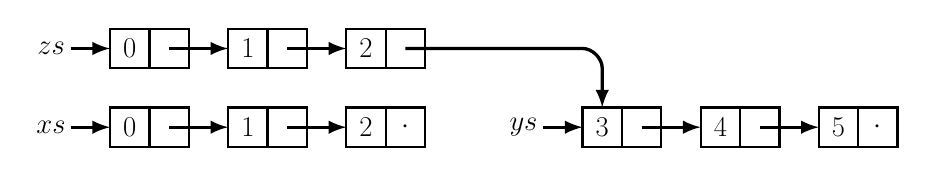
\begin{tikzpicture}[thick,scale=0.5, every node/.style={scale=0.5}]
    \tikzstyle{marrs}=[very thick,-latex]
    
    
    
    \begin{scope}
    
        \foreach \x/\y in {0/0, 3/0, 6/0} {
            \draw (\x - 0.5, \y - 0.5) rectangle +(1, 1); \draw (\x + 1 - 0.5, \y - 0.5) rectangle +(1, 1);
        }
        \draw[marrs] (-1.5, 0) -> +(1, 0);
        \draw[marrs] (1, 0) -> +(1.5, 0);
        \draw[marrs] (4, 0) -> +(1.5, 0);
        
        { \huge
            \draw (-2, 0) node {$xs$};
            \draw (0, 0) node {$0$};
            \draw (3, 0) node {$1$};
            \draw (6, 0) node {$2$};
            \draw (7, 0) node {$\cdot$};
        }
    
    \end{scope}
    
    \begin{scope}[xshift=12cm]
    
        \foreach \x/\y in {0/0, 3/0, 6/0} {
            \draw (\x - 0.5, \y - 0.5) rectangle +(1, 1); \draw (\x + 1 - 0.5, \y - 0.5) rectangle +(1, 1);
        }
        \draw[marrs] (-1.5, 0) -> +(1, 0);
        \draw[marrs] (1, 0) -> +(1.5, 0);
        \draw[marrs] (4, 0) -> +(1.5, 0);
        
        { \huge
            \draw (-2, 0) node {$ys$};
            \draw (0, 0) node {$3$};
            \draw (3, 0) node {$4$};
            \draw (6, 0) node {$5$};
            \draw (7, 0) node {$\cdot$};
        }
    \end{scope}
    
    \begin{scope}[yshift=2cm]
    
        \foreach \x/\y in {0/0, 3/0, 6/0} {
            \draw (\x - 0.5, \y - 0.5) rectangle +(1, 1); \draw (\x + 1 - 0.5, \y - 0.5) rectangle +(1, 1);
        }
        \draw[marrs] (-1.5, 0) -> +(1, 0);
        \draw[marrs] (1, 0) -> +(1.5, 0);
        \draw[marrs] (4, 0) -> +(1.5, 0);
        
        { \huge
            \draw (-2, 0) node {$zs$};
            \draw (0, 0) node {$0$};
            \draw (3, 0) node {$1$};
            \draw (6, 0) node {$2$};
            
            \draw[marrs] (7, 0) -- (11.5, 0) .. controls (11.75, 0) and (12, -0.25) .. (12, -0.5) -- (12, -1.5);
        }
    
    \end{scope}
    
    
    
\end{tikzpicture}\par
	(после)\par
	\vspace{0.5cm}
	\caption{Выполнение \texttt{zs = xs ++ ys} в функциональной среде. Заметим, что списки-аргументы \texttt{xs} и \texttt{ys} не затронуты операцией.
	}
	\label{fig:2.5}
\end{figure}
Несмотря на большой объем копирования, заметим, что второй список копировать не пришлось
\end{frame}

\begin{frame}[fragile]{Update}
\inputminted[firstline=60,lastline=64] {haskell}{code/Stacks.hs}
%Если нам доступно внутреннее представление, то можно написать более короткий идиоматичный код
Здесь мы не копируем весь список-аргумент.\\

Копировать приходится
только сам узел, подлежащий модификации (узел $i$) и узлы,
содержащие прямые или косвенные указатели на $i$. \\

Другими словами,
чтобы изменить один узел, мы копируем все узлы на пути от корня
к изменяемому. Все узлы, не находящиеся на этом пути, используются как
исходной, так и обновленной версиями. 
%На Рис.
%~\ref{fig:2.6} 
%показан
%результат изменения третьего узла в пятиэлементном списке: первые
%три узла копируются, а последние два используются совместно.
\end{frame}

\begin{frame}[fragile]{}
\begin{figure}[h]
	\centering
	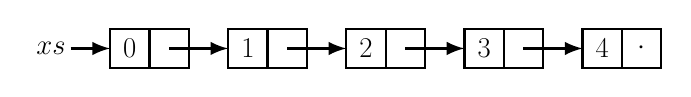
\begin{tikzpicture}[thick,scale=0.5, every node/.style={scale=0.5}]
    \tikzstyle{marrs}=[very thick,-latex]

    \begin{scope}
    
        \foreach \x/\y in {0/0, 3/0, 6/0, 9/0, 12/0} {
            \draw (\x - 0.5, \y - 0.5) rectangle +(1, 1); \draw (\x + 1 - 0.5, \y - 0.5) rectangle +(1, 1);
        }
        \draw[marrs] (-1.5, 0) -> +(1, 0);
        \foreach \x in {1, 4, 7, 10} {
            \draw[marrs] (\x, 0) -> +(1.5, 0);
        }
        
        { \huge
            \draw (-2, 0) node {$xs$};
            \foreach \x/\y in {0/0, 3/1, 6/2, 9/3, 12/4} {
                \draw (\x, 0) node {$\y$};
            }
            \draw (13, 0) node {$\cdot$};
        }
    
    \end{scope}
    
\end{tikzpicture}\par
	(до)\par
	\vspace{0.5cm}
	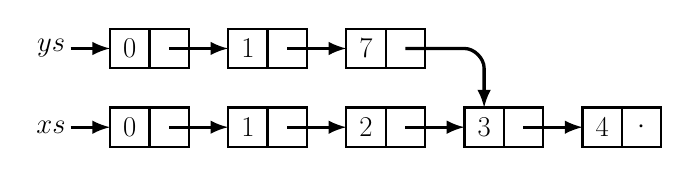
\begin{tikzpicture}[thick,scale=0.5, every node/.style={scale=0.5}]
    \tikzstyle{marrs}=[very thick,-latex]
    
    
    
    \begin{scope}
    
        \foreach \x/\y in {0/0, 3/0, 6/0, 9/0, 12/0} {
            \draw (\x - 0.5, \y - 0.5) rectangle +(1, 1); \draw (\x + 1 - 0.5, \y - 0.5) rectangle +(1, 1);
        }
        \draw[marrs] (-1.5, 0) -> +(1, 0);
        \foreach \x in {1, 4, 7, 10} {
            \draw[marrs] (\x, 0) -> +(1.5, 0);
        }
        
        { \huge
            \draw (-2, 0) node {$xs$};
            \foreach \x/\y in {0/0, 3/1, 6/2, 9/3, 12/4} {
                \draw (\x, 0) node {$\y$};
            }
            \draw (13, 0) node {$\cdot$};
        }   
    
    \end{scope}
    
    \begin{scope}[yshift=2cm]
    
        \foreach \x/\y in {0/0, 3/0, 6/0} {
            \draw (\x - 0.5, \y - 0.5) rectangle +(1, 1); \draw (\x + 1 - 0.5, \y - 0.5) rectangle +(1, 1);
        }
        \draw[marrs] (-1.5, 0) -> +(1, 0);
        \draw[marrs] (1, 0) -> +(1.5, 0);
        \draw[marrs] (4, 0) -> +(1.5, 0);
        
        { \huge
            \draw (-2, 0) node {$ys$};
            \draw (0, 0) node {$0$};
            \draw (3, 0) node {$1$};
            \draw (6, 0) node {$7$};
            
            \draw[marrs] (7, 0) -- (8.5, 0) .. controls (8.75, 0) and (9, -0.25) .. (9, -0.5) -- (9, -1.5);
        }
    
    \end{scope}
    
    
    
\end{tikzpicture}\par
	(после)\par
	\vspace{0.5cm}	
	\caption{Выполнение \texttt{ys = update xs 2 7}. Обратите
		внимание на совместное использование структуры списками \texttt{xs} и \texttt{ys}.}
	\label{fig:2.6}
\end{figure}
\end{frame}

\begin{frame}[fragile]
\begin{remark}
	Такой стиль программирования очень сильно упрощается при наличии
	автоматической сборки мусора. Очень важно освободить память от тех
	копий, которые больше не нужны, но многочисленные совместно используемые
	узлы делают ручную сборку мусора нетривиальной задачей.
\end{remark}
\begin{exercise}\label{ex:2.1}
  Напишите функцию \texttt{suffixes} типа \mintinline{haskell}{[a] -> [a]}, которая принимает как
  аргумент список \texttt{xs} и возвращает список всех его
  суффиксов в убывающем порядке длины. Например,
  \begin{minted}{haskell}
  suffixes [1,2,3,4] = [[1,2,3,4],[2,3,4],[3,4],[4],[]]
  \end{minted}
  Покажите, что список суффиксов можно породить за время $O(n)$ и
  занять при этом $O(n)$ памяти.
\end{exercise}

\end{frame}

\section{Двоичные деревья поиска}
\label{sc:2.2}

\begin{frame}{Двоичные деревья поиска}
Если узел структуры содержит более одного указателя, оказываются
возможны более сложные сценарии совместного использования памяти. Хорошим примером
совместного использования такого вида служат \emph{двоичные деревья поиска}.

\inputminted[firstline=10, lastline=10] {haskell}{code/SearchTree.hs}

Двоичные деревья поиска~--- это двоичные деревья, в которых элементы
хранятся во внутренних узлах в \term{симметричном}{symmetric}
порядке, то есть, элемент в каждом узле больше любого элемента в
левом поддереве этого узла и меньше любого элемента в правом
поддереве.
\end{frame}

\begin{frame}[fragile]{}
\begin{figure}[h]
  \centering
  \inputminted[firstline=12, lastline=15]{haskell}{code/SearchTree.hs}
  \caption{Сигнатура для множеств.}
\label{fig:2.7}
\end{figure}

Cигнатура для множеств значение <<пустое множество>>, а также функции добавления
нового элемента и проверки на членство.  В более практической
реализации, вероятно, будут присутствовать и многие другие функции,
например, для удаления элемента или перечисления всех элементов.
\end{frame}

\begin{frame}[fragile]{Функция \hsinline{member}}
Ищет в дереве, сравнивая запрошенный элемент с находящимся в корне дерева. 
\inputminted[firstline=22, lastline=25] {haskell}{code/SearchTree.hs}


Если мы когда-либо натыкаемся на пустое дерево, значит,
запрашиваемый элемент не является членом множества, и мы возвращаем
значение <<ложь>>. \\

Если запрошенный элемент \textbf{меньше}
корневого, мы рекурсивно ищем в левом поддереве.

Если он \textbf{больше}, рекурсивно ищем в правом поддереве. 

Наконец, в оставшемся случае
запрошенный элемент \textbf{равен} корневому, и мы возвращаем значение
<<истина>>. 
\end{frame}

\begin{frame}[fragile]{Функция insert}
\inputminted[firstline=27, lastline=31] {haskell}{code/SearchTree.hs}

Функция \hsinline{insert} проводит поиск в дереве по той же стратегии,
что и \hsinline{member}, но только по пути она копирует каждый
элемент. \\

Когда, наконец, оказывается достигнут пустой узел, он
заменяется на узел, содержащий новый элемент.
 
\end{frame}

\begin{frame}[fragile]{}
\begin{minipage}{.48\textwidth}
		\documentclass[tikz]{standalone}
%\usepackage{fontawesome}

% \newfontfamily{\FA}{Font Awesome 5 Free} % some glyphs missing
\expandafter\def\csname faicon@facebook\endcsname{{\FA\symbol{"F09A}}}
\def\faQuestionSign{{\FA\symbol{"F059}}}
\def\faQuestion{{\FA\symbol{"F128}}}
\def\faExclamation{{\FA\symbol{"F12A}}}
\def\faUploadAlt{{\FA\symbol{"F093}}}
\def\faLemon{{\FA\symbol{"F094}}}
\def\faPhone{{\FA\symbol{"F095}}}
\def\faCheckEmpty{{\FA\symbol{"F096}}}
\def\faBookmarkEmpty{{\FA\symbol{"F097}}}

%\def\faCatt{{\FA\symbol{"F6BE}}}
%\def\faCat{\faicon{cat}}
%\def\faCat{\faicon{yoast}}
\expandafter\def\csname faicon@dog\endcsname{{\FA\symbol{"F4DA}}}
%\def\faDog{\faicon{dog}}
%\def\faDog{{\FA\symbol{"F4DA}}}
%\def\faDogg{{\FA\symbol{"F6D3}}}
%\def\faDogg{{\FA\symbol{"F596}}}

% /usr/share/texlive/texmf-dist/fonts/opentype/public/fontawesome5/FontAwesome5Free-Solid-900.otf
\newfontfamily{\FAS}{FontAwesome5Free-Solid-900.otf}
%\expandafter\def\csname faicon@download\endcsname{{\FAS\symbol{"F6D3}}}
\expandafter\def\csname faicon@cat\endcsname{{\FAS\symbol{"F6BE}}}
\def\faCat{\faicon{cat}}
\expandafter\def\csname faicon@dog\endcsname{{\FAS\symbol{"F6D3}}}
\def\faDog{\faicon{dog}}
\expandafter\def\csname faicon@dragon\endcsname{{\FAS\symbol{"F6D5}}}
\def\faDragon{\faicon{dragon}}
\expandafter\def\csname faicon@fish\endcsname{{\FAS\symbol{"F578}}}
\def\faFish{\faicon{fish}}
\expandafter\def\csname faicon@horse\endcsname{{\FAS\symbol{"F6F0}}}
\def\faHorse{\faicon{horse}}
\expandafter\def\csname faicon@spider\endcsname{{\FAS\symbol{"F717}}}
\def\faSpider{\faicon{spider}}

\expandafter\def\csname faicon@chessking\endcsname{{\FAS\symbol{"F43F}}}
\def\faChessKing{\faicon{chessking}}
\expandafter\def\csname faicon@chessqueen\endcsname{{\FAS\symbol{"F445}}}
\def\faChessQueen{\faicon{chessqueen}}
\expandafter\def\csname faicon@chessrook\endcsname{{\FAS\symbol{"F447}}}
\def\faChessRook{\faicon{chessrook}}
\expandafter\def\csname faicon@chesspawn\endcsname{{\FAS\symbol{"F443}}}
\def\faChessPawn{\faicon{chesspawn}}
\expandafter\def\csname faicon@chessknight\endcsname{{\FAS\symbol{"F441}}}
\def\faChessKnight{\faicon{chessknight}}
\expandafter\def\csname faicon@chessbishop\endcsname{{\FAS\symbol{"F43A}}}
\def\faChessBishop{\faicon{chessbishop}}
\expandafter\def\csname faicon@chess\endcsname{{\FAS\symbol{"F439}}}
\def\faChess{\faicon{chess}}







\usepackage{tikz}
\usetikzlibrary{positioning,trees,decorations.pathreplacing}

\begin{document}
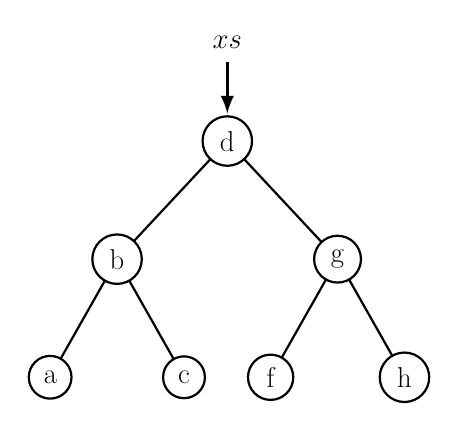
\begin{tikzpicture}[thick,scale=0.5, every node/.style={scale=0.5},level distance=3cm]
    \tikzstyle{marrs}=[very thick,-latex]
    \tikzstyle{tnode}=[circle, draw=black,node distance=1.7cm]
    \tikzstyle{level 1}=[sibling distance=5.6cm]
    \tikzstyle{level 2}=[sibling distance=3.4cm]


    \huge

    \draw (0, 2.5) node {$xs$};
    \draw[marrs] (0, 2) -- (0, 0.7);
    \node[tnode] {d}
    child {node[tnode] {b}
        child {node[tnode] {a}}
        child {node[tnode] {c}}
    }
    child {node[tnode] {g}
        child {node[tnode] {f}}
        child {node[tnode] {h}}
    };
    
\end{tikzpicture}
\end{document}\par
\end{minipage}
\begin{minipage}{.48\textwidth}
	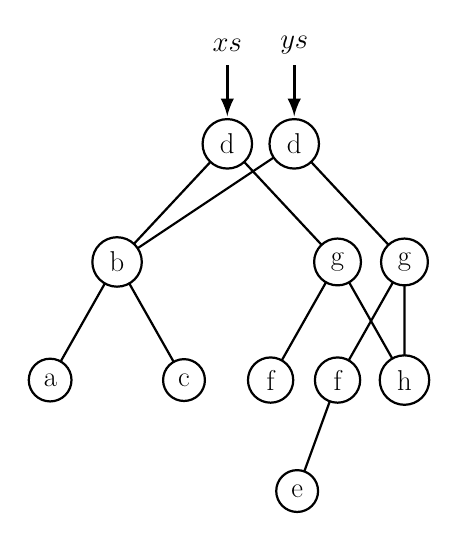
\begin{tikzpicture}[thick,scale=0.5, every node/.style={scale=0.5},level distance=3cm]
    \tikzstyle{marrs}=[very thick,-latex]
    \tikzstyle{tnode}=[circle, draw=black,node distance=1.7cm]
    \tikzstyle{level 1}=[sibling distance=5.6cm]
    \tikzstyle{level 2}=[sibling distance=3.4cm]
    
    \huge

    \draw (0, 2.5) node {$xs$};
    \draw[marrs] (0, 2) -- +(0, -1.3);
    
    \draw (1.7, 2.5) node {$ys$};
    \draw[marrs] (1.7, 2) -- +(0, -1.3);
    
    \node[tnode] (n_d) {d}
    child {node[tnode] (n_b) {b}
        child {node[tnode] (n_a) {a}}
        child {node[tnode] (n_c) {c}}
    }
    child {node[tnode] (n_g) {g}
        child {node[tnode] (n_f) {f}
        node[tnode] (n_f') [right of=n_f] {f} [clockwise from=250]
        child {node[tnode] (n_e) {e}}
        }
        child {node[tnode] (n_h) {h}}
        node[tnode] (n_g') [right of=n_g] {g}
    }
    node[tnode] (n_d') [right of=n_d]{d};
    
    \path (n_d') edge (n_b);
    \path (n_d') edge (n_g');
    \path (n_g') edge (n_f');
    \path (n_g') edge (n_h);
    
\end{tikzpicture}
\end{minipage}
Выполнение \texttt{ys = insert "e" xs}. 
%Как и прежде,
%обратите внимание на совместное использвание структуры деревьями \texttt{xs} и \texttt{ys}.

%Каждый скопированный узел использует одно из поддеревьев 
%совместно с исходным деревом; речь о том поддереве,
%которое не оказалось на пути поиска. 
Для большинства деревьев путь
поиска содержит лишь небольшую долю узлов в дереве. Громадное
большинство узлов находятся в совместно используемых поддеревьях.
\end{frame}

\begin{frame}
\begin{exercise}\textbf{Андерсон \cite{Andersson1991}}\label{ex:2.2}
  В худшем случае \lstinline{member} производит $2d$ сравнений, где
  $d$~--- глубина дерева. Перепишите ее так, чтобы она делала не более
  $d+1$ сравнений, сохраняя элемент, который \emph{может} оказаться
  равным запрашиваемому (например, последний элемент, для которого
  операция $<$ вернула значение <<истина>> или $\le$~--- <<ложь>>, и
  производя проверку на равенство только по достижении дна дерева.
\end{exercise}

\begin{exercise}\label{ex:2.3}
  Вставка уже существующего элемента в двоичное дерево поиска копирует
  весь путь поиска, хотя скопированные узлы неотличимы от
  исходных. Перепишите \lstinline{insert} так, чтобы она избегала
  копирования с помощью исключений. Установите только один обработчик
  исключений для всей операции поиска, а не по обработчику на итерацию.
\end{exercise}
\end{frame}

\ifanswers
\begin{frame}
\begin{exercise}\label{ex:2.4}
  Совместите улучшения из предыдущих двух упражнений, и получите
  версию \lstinline{insert}, которая не делает ненужного копирования и
  использует не более $d+1$ сравнений.
\end{exercise}
\end{frame}

\begin{frame}
\begin{exercise}\label{ex:2.5}
  Совместное использование может быть полезно и внутри одного объекта, не
  обязательно между двумя различными.  Например, если два поддерева
  одного дерева идентичны, их можно представить одним и тем же
  деревом.
  \begin{enumerate}
    \item Используя эту идею, напишите функцию \lstinline{complete} типа
    \mintinline{haskell}{Elem -> Int -> Tree}, такую, что
    \mintinline{haskell}{complete(x,d)} создает полное двоичное дерево глубины
    \lstinline{d}, где в каждом узле содержится \lstinline{x}.
    (Разумеется, такая функция бессмысленна для абстракции множества,
    но она может оказаться полезной для какой-либо другой абстракции,
    например, мультимножества.) Функция должна работать за время $O(d)$.
    \item Расширьте свою функцию, чтобы она строила сбалансированные
    деревья произвольного размера. Эти деревья не всегда будут полны,
    но они должны быть как можно более сбалансированными: для любого
    узла размеры поддеревьев должны различаться не более чем на
    единицу. Функция должна работать за время $O(\log n)$. (Подсказка:
    воспользуйтесь вспомогательной функцией \lstinline{create2},
    которая, получая размер $m$, создает пару деревьев~--- одно размера
    $m$, а другое размера $m+1$)
  \end{enumerate}
\end{exercise}
\end{frame}


\begin{frame}
\begin{exercise}\label{ex:2.6}
  Измените функтор \texttt{UnbalancedSet} так, чтобы он служил
  реализацией не множеств, а \term{конечных отображений}{finite maps}. На
  Рис.~\ref{fig:2.10} приведена минимальная сигнатура для конечных
  отображений. (Заметим, что исключение \texttt{NotFound} не
  является встроенным в Стандартный ML~--- Вам придется его определить
  самостоятельно. Это исключение можно было бы сделать частью
  сигнатуры \texttt{FiniteMap},  чтобы каждая реализация
  определяла собственное исключение \texttt{NotFound}, но удобнее,
  если все конечные отображения будут использовать одно и то же
  исключение.)
\end{exercise}
\end{frame}
\fi 

\section{Левоориентированные кучи}

\begin{frame}[fragile]{}
Как правило, множества и конечные отображения поддерживают эффективный
доступ к произвольным элементам. Однако иногда требуется эффективный
доступ только к \emph{минимальному} элементу.  Структура данных,
поддерживающая такой режим доступа, называется \term{очередь с
приоритетами}{priority queue} или \term{куча}{heap}.

\inputminted[firstline=4, lastline=12] {haskell}{code/Heap.hs}
\end{frame}

\begin{frame}[fragile]{}
Часто кучи реализуются через деревья \term{с порядком
  кучи}{heap-ordered}, т.~е., в которых элемент при каждой вершине не
больше элементов в поддеревьях. При таком упорядочении минимальный
элемент дерева всегда находится в корне.\vspace{1cm}

Левоориентированные кучи \cite{Crane1972, Knuth1973a} представляют
собой двоичные деревья с порядком кучи, обладающие свойством
\term{левоориентированности}{leftist property}: ранг любого левого поддерева
не меньше ранга его сестринской правой вершины.  Ранг узла
определяется как длина его \term{правой периферии}{right spine}
(т.~е., самого правого пути от данного узла до пустого).  Простым
следствием свойства левоориентированности является то, что правая
периферия любого узла~--- кратчайший путь от него к пустому узлу.
\end{frame}

\begin{frame}[fragile]{Левоориентированные кучи}
Если у нас есть некоторый тип упорядоченных элементов
\mintinline{haskell}{e}, 
мы можем представить левоориентированные кучи как
двоичные деревья, снабженные информацией о ранге.
\inputminted[firstline=18, lastline=18] {haskell}{code/Heap.hs}

Заметим, что элементы правой периферии левоориентированной кучи (да и
любого дерева с порядком кучи) расположены в порядке возрастания.\\

Главная идея левоориентированной кучи заключается в том, что для
слияния двух куч достаточно слить их правые периферии как
упорядоченные списки, а затем вдоль полученного пути обменивать
местами поддеревья при вершинах, чтобы восстановить свойство
левоориентированности. 

\end{frame}

\begin{frame}[fragile]{}
\inputminted[firstline=23, lastline=26] {haskell}{code/Heap.hs}

где \hsinline{makeT}~--- вспомогательная функция, вычисляющая ранг
вершины \hsinline{T} и, если необходимо, меняющая местами ее
поддеревья.

\inputminted[firstline=30, lastline=35] {haskell}{code/Heap.hs}

Поскольку длина правой периферии любой вершины в худшем случае
логарифмическая, \hsinline{merge} выполняется за время $O(\log n)$.
\end{frame}

\begin{frame}[fragile]{}
\inputminted[firstline=36, lastline=38] {haskell}{code/Heap.hs}

Поскольку \hsinline{merge} выполняется за время $O(\log n)$, столько
же занимают и \hsinline{insert} с \hsinline{deleteMin}.\\

Очевидно, что \hsinline{findMin} выполняется за $O(1)$. 
\end{frame}

\ifanswers
\begin{frame}[fragile]{}
\begin{exercise}\label{ex:3.2}
  Определите \hsinline{insert} напрямую, а не через обращение к \hsinline{merge}.
\end{exercise}

\begin{exercise}\label{ex:3.3}
  Реализуйте функцию \hsinline{fromList} типа \hsinline{Elem.T list $\to$ Heap},
  порождающую левоориентированную кучу из неупорядоченного списка
  элементов путем преобразования каждого элемента в одноэлементную
  кучу, а затем слияния получившихся куч, пока не останется
  одна. Вместо того, чтобы сливать кучи проходом слева направо или
  справа налево при помощи \hsinline{foldr} или \hsinline{foldl},
  слейте кучи за $\lceil \log n \rceil$ проходов, где на каждом
  проходе сливаются пары соседних куч. Покажите, что
  \hsinline{fromList} требует всего $O(n)$ времени.
\end{exercise}
\end{frame}
\fi 

\begin{frame}[fragile]{}
\begin{exercise}\label{ex:3.4}
  Левоориентированные кучи
  со сдвинутым весом~--- альтернатива левоориентированным кучам, где
  вместо свойства левоориентированности используется свойство
  \term{левоориентированности, сдвинутой по весу}{weight-biased leftist
    property}: размер любого левого поддерева всегда не меньше размера
  соответствующего правого поддерева.
  \begin{enumerate}
    \item Докажите, что правая периферия левоориентированной кучи со
    сдвинутым весом содержит не более $\lfloor \log(n+1) \rfloor$ элементов.
    \item Измените реализацию, чтобы получились
    левоориентированные кучи со сдвинутым весом.
    \item Функция \lstinline!merge! сейчас выполняется в два прохода:
    сверху вниз, с вызовами \lstinline!merge!, и снизу вверх, с
    вызовами вспомогательной функции \lstinline!makeT!. Измените
    \lstinline!merge! для левоориентированных куч со сдвинутым весом
    так, чтобы она работала за один проход сверху вниз.
    \item Каковы преимущества однопроходной версии в
    условиях ленивого вычисления? Параллельного?
  \end{enumerate}
\end{exercise}

\end{frame}

\section{Биномиальные кучи}
\label{sc:3.2}

\begin{frame}{Биномиальные кучи}
Биномиальные очереди \cite{Vuillemin1978, Brown1978}, которые мы,
чтобы избежать путаницы с очередями FIFO, будем называть \term{ биномиальными
  кучами}{binomial heaps}~--- ещё одна распространенная реализация
куч. \\

Биномиальные кучи устроены сложнее, чем левоориентированные, и, на
первый взгляд, не возмещают эту сложность никакими
преимуществами. \\

Однако, с помощью дополнительных хитростей (амортизация\cite{sc:5.3}), можно заставить \hsinline{insert} и
\hsinline{merge} выполняться за время $O(1)$.



\end{frame}

\begin{frame}{Биномиальные деревья}
Биномиальные кучи строятся из более простых объектов, называемых
биномиальными деревьями. Биномиальные деревья индуктивно определяются
так:
\begin{itemize}
  \item Биномиальное дерево ранга 0 представляет собой одиночный узел.
  \item Биномиальное дерево ранга $r+1$ получается путем
  \term{связывания}{linking} двух биномиальных деревьев ранга $r$, так
  что одно из них становится самым левым потомком второго.
\end{itemize}
Из этого определения видно, что биномиальное дерево ранга $r$ содержит
ровно $2^r$ элементов.  \\

Существует второе, эквивалентное первому,
определение биномиальных деревьев, которым иногда удобнее
пользоваться: биномиальное дерево ранга $r$ представляет собой узел
с $r$ потомками $t_1\ldots t_r$, где каждое $t_i$ является
биномиальным деревом ранга $(r-i)$.
\end{frame}


\begin{frame}[fragile]{}
\begin{figure}[h]
  \centering
  \begin{tikzpicture}[thick,scale=0.5, every node/.style={scale=0.5},grow via three points={%
one child at (0,-1.5) and two children at (0,-1.5) and (-0.8,-1.5)}
]
    \tikzstyle{marrs}=[very thick,-latex]
    \tikzstyle{tnode}=[circle, fill=black, inner sep=1.5mm]
    \def\rstep{5cm}
    
    \huge
    
    \node[tnode] (0, 0) {};
            child { node[tnode] {} }
            child { node[tnode] {} };
    
    \begin{scope}
        \draw (0, 1) node {Ранг 0};
        \node[tnode] (0, 0) {};
    \end{scope}
    
    \begin{scope}[xshift=\rstep]
        \draw (0, 1) node {Ранг 1};
        \node[tnode] {}
            child {node[tnode] {} };
    \end{scope}
    
    \begin{scope}[xshift=2 * \rstep]
        \draw (0, 1) node {Ранг 2};
        \node[tnode] {}
            child {node[tnode] {} }
            child {node[tnode] {} 
                    child {node[tnode] {} }};
            
            
    \end{scope}
    
    \begin{scope}[xshift=3 * \rstep]
        \draw (0, 1) node {Ранг 3};
        \node[tnode] {}
            child {node[tnode] {} }
            child {node[tnode] {} 
                child {node[tnode] {} }
            }
            child {node[tnode] {} 
                child {node[tnode] {} }
                child {node[tnode] {} 
                    child {node[tnode] {} }
                }
          };
            
            
    \end{scope}
    
    
\end{tikzpicture}

  \caption{Биномиальные деревья рангов 0--3.}
  \label{fig:3.3}
\end{figure}

%\inputminted[firstline=5, lastline=6] {haskell}{code/BinomialHeap.lhs}

\end{frame}


\begin{frame}[fragile]{}
\inputminted[firstline=5, lastline=5] {haskell}{code/BinomialHeap.lhs}

Каждый список потомков хранится в \emph{убывающем} (sic!) порядке рангов, а элементы
хранятся вместе с рангом кучи.  Чтобы сохранять этот порядок рангов, мы всегда
привязываем дерево с большим корнем к дереву с меньшим.

\inputminted[firstline=11, lastline=15] {haskell}{code/BinomialHeap.lhs}

Будем привязывать деревья только с одинаковым рангом
\end{frame}


\begin{frame}[fragile]{}
Определяем биномиальную кучу как 
\begin{itemize}
  \item коллекцию биномиальных деревьев
  \item каждое из которых имеет порядок кучи
  \item никакие два дерева не совпадают по рангу
\end{itemize} 

Например, список деревьев в порядке возрастания ранга.
\inputminted[firstline=6, lastline=6] {haskell}{code/BinomialHeap.lhs}
\end{frame}


\begin{frame}[fragile]{Биномиальные кучи и числа}
Поскольку каждое биномиальное дерево содержит $2^r$ элементов, и
никакие два дерева по рангу не совпадают, деревья размера $n$ в
точности соответствуют единицам в двоичном представлении
$n$.\\

Например, число $21_{10} = 10101_2$, и поэтому
биномиальная куча размера 21 содержит одно дерево ранга 0, одно ранга
2, и одно ранга 4 (размерами, соответственно, 1, 4 и 16).\\

Заметим, что
так же, как двоичное представление $n$ содержит не более $\lfloor log
(n+1)\rfloor$ единиц, биномиальная куча размера $n$ содержит не более
$\lfloor log(n+1) \rfloor$ деревьев.
\end{frame}


\begin{frame}[fragile]{}
\begin{figure}[h]
  \centering
  \begin{tikzpicture}[thick,scale=0.5, every node/.style={scale=0.5},grow via three points={%
one child at (0,-1.5) and 
two children at (0,-1.5) and (-0.8,-1.5) 
}
]
    \tikzstyle{marrs}=[very thick,-latex]
    \tikzstyle{tnode}=[circle, fill=black, inner sep=1.5mm]
    \def\rstep{5cm}
    
    \huge
    
    \node[tnode] (0, 0) {};
            child { node[tnode] {} }
            child { node[tnode] {} };
    
    \begin{scope}
        \draw (0, 1) node {Ранг 0};
        \node[tnode] (0, 0) {};
    \end{scope}
        
    \begin{scope}[xshift=1 * \rstep]
        \draw (0, 1) node {Ранг 2};
        \node[tnode] {}
            child {node[tnode] {} }
            child {node[tnode] {} 
                    child {node[tnode] {} }};
    \end{scope}
    
    \begin{scope}[xshift=3 * \rstep]
      \draw (0, 1) node {Ранг 4};
      \node[tnode] {}
          child {node[tnode] {} }
          child {node[tnode] {} 
            child {node[tnode] {} }
          }
          child {node[tnode] {} 
            child {node[tnode] {} }
            child {node[tnode] {} 
              child {node[tnode] {} }
            }
          }
        child[missing] {}
        child {node[tnode] {}
          child {node[tnode] {} }
          child {node[tnode] {} 
            child {node[tnode] {} }
          }
          child {node[tnode] {} 
            child {node[tnode] {} }
            child {node[tnode] {} 
              child {node[tnode] {} }
            }
          }
     };
      \end{scope}
    
    
\end{tikzpicture}

  \caption{Число $21_{10} = 10101_2$, и поэтому
    биномиальная куча размера 21 содержит одно дерево ранга 0, одно ранга
    2, и одно ранга 4 (размерами, соответственно, 1, 4 и 16).}
\end{figure}

\end{frame}


\begin{frame}[fragile]{\hsinline{insert} -- аналогично сложению}
% (Мы укрепим эту аналогию в Главе~\ref{ch:9}.). \\

Чтобы внести элемент в кучу,
мы сначала создаем одноэлементное дерево (т.~е., биномиальное дерево
ранга 0), затем поднимаемся по списку существующих деревьев в порядке
возрастания рангов, связывая при этом одноранговые деревья. Каждое
связывание соответствует переносу в двоичной арифметике.

\inputminted[firstline=8,lastline=8] {haskell}{code/BinomialHeap.lhs}
\inputminted[firstline=17,lastline=19] {haskell}{code/BinomialHeap.lhs}
\inputminted[firstline=38,lastline=38,gobble=2] {haskell}{code/BinomialHeap.lhs}
В худшем случае, при вставке в кучу размера $n = 2^k -1$, требуется
$k$ связываний и $O(k) = O(\log n)$ времени.
\end{frame}


\begin{frame}[fragile]{\hsinline{merge} -- аналогично сложению}
При слиянии двух куч мы проходим через оба списка деревьев в порядке
возрастания ранга и связываем по пути деревья равного ранга. Как и
прежде, каждое связывание соответствует переносу в двоичной
арифметике.

\inputminted[firstline=21,lastline=26] {haskell}{code/BinomialHeap.lhs}

\inputminted[firstline=39,lastline=39,gobble=2] {haskell}{code/BinomialHeap.lhs}

\end{frame}

\begin{frame}[fragile]{}
Функции \hsinline{findMin} и \hsinline{deleteMin} вызывают
вспомогательную функцию \hsinline{removeMinTree}, которая находит
дерево с минимальным корнем, исключает его из списка и возвращает как
это дерево, так и список оставшихся деревьев.

\inputminted[firstline=28,lastline=32]{haskell}{code/BinomialHeap.lhs}

Функция \hsinline{findMin} просто возвращает корень найденного дерева

\inputminted[firstline=40,lastline=41,gobble=2] {haskell}{code/BinomialHeap.lhs}
\inputminted[firstline=9,lastline=9] {haskell}{code/BinomialHeap.lhs}
\end{frame}

\begin{frame}[fragile]{}
Функция \hsinline{deleteMin} устроена немного похитрее. \\

 Отбросив
корень найденного дерева, мы ещё должны вернуть его потомков в список
остальных деревьев. Заметим, что список потомков \emph{почти} уже
соответствует определению биномиальной кучи. Это коллекция
биномиальных деревьев с неповторяющимися рангами, но только
отсортирована она не по возрастанию, а по убыванию ранга. Таким
образом, обратив список потомков, мы преобразуем его в биномиальную
кучу, а затем сливаем с оставшимися деревьями.

\inputminted[firstline=43,lastline=44,gobble=2] {haskell}{code/BinomialHeap.lhs}
\end{frame}

\ifanswers
\begin{frame}[fragile]{}
\begin{exercise}\label{ex:3.5}
  Определите \lstinline!findMin! напрямую, без обращения к \lstinline!removeMinTree!.
\end{exercise}

\begin{exercise}\label{ex:3.6}
  Большая часть аннотаций ранга в нашем представлении биномиальных куч
  излишня, потому что мы и так знаем, что дети узла ранга $r$ имеют
  ранги $(r\!-\!1), \ldots, 0$. Таким образом, можно исключить
  поле-аннотацию ранга из узлов, а вместо этого помечать ранг корня
  каждого дерева, т.~е.,
  \begin{minted}{haskell}
  data Tree a = Node  a [Tree]
  type Heap = [(Int, Tree)]
  \end{minted}
  Реализуйте биномиальные кучи в таком представлении.
\end{exercise}
\end{frame}

% Ещё одно упражнение не скопипастьил

\fi

\section{Красно-чёрные деревья}
\label{sc:3.3}

\begin{frame}[fragile]{Красно-чёрные деревья}
Двоичные деревья поиска хорошо ведут себя на случайных или неупорядоченных данных,
однако на упорядоченных данных их производительность резко падает, и
каждая операция может занимать до $O(n)$  времени. \\

 Решение этой
проблемы состоит в том, чтобы каждое дерево поддерживать в
приблизительно сбалансированном состоянии. Тогда каждая операция
выполняется не хуже, чем за время $O(\log n)$. \\

 Одним из наиболее
популярных семейств сбалансированных двоичных деревьев поиска являются
красно-чёрные \cite{GuibasSedgewick1978}.
\end{frame}

\begin{frame}[fragile]{}
Красно-чёрное дерево представляет собой двоичное дерево поиска, в
котором каждый узел окрашен либо красным, либо чёрным. Мы добавляем
поле цвета в тип двоичных деревьев поиска %из раздела~\ref{sc:2.2}.

\inputminted[firstline=6,lastline=7] {haskell}{code/RedBlackSet.lhs}
Все пустые узлы считаются чёрными, поэтому пустой конструктор
\hsinline{E} в поле цвета не нуждается.

\end{frame}

\begin{frame}[fragile]{Красно-чёрные деревья. Инварианты}
Мы требуем, чтобы всякое красно-чёрное дерево соблюдало два
инварианта:
\begin{itemize}
  \item \textbf{Инвариант 1.} У красного узла не может быть красного ребёнка.
  \item \textbf{Инвариант 2.} Каждый путь от корня дерева до пустого
  узла содержит одинаковое количество чёрных узлов.
\end{itemize}
Вместе эти два инварианта гарантируют, что самый длинный возможный
путь по красно-чёрному дереву, где красные и чёрные узлы чередуются,
не более чем вдвое длиннее самого короткого, состоящего только из
чёрных узлов.

\ifanswers
\begin{exercise}\label{ex:3.8}
  Докажите, что максимальная глубина узла в красно-чёрном дереве
  размера $n$ не превышает $2 \lfloor \log (n+1) \rfloor$.
\end{exercise}
\fi
\end{frame}

\begin{frame}[fragile]{}
Функция \hsinline{member} для красно-чёрных деревьев не обращает
внимания на цвета. За исключением wildcard в варианте для конструктора
\hsinline{T}, она не отличается от функции \hsinline{member} для
несбалансированных деревьев.
\inputminted[firstline=18,lastline=21] {haskell}{code/RedBlackSet.lhs}
\end{frame}


\begin{frame}[fragile]{}
Функция \hsinline{insert} интереснее: она должна
поддерживать два инварианта балансировки.

\inputminted[firstline=23,lastline=29] {haskell}{code/RedBlackSet.lhs}

Эта функция содержит три существенных изменения по сравнению с \hsinline{insert} для
несбалансированных деревьев поиска. Во-первых, когда мы создаем новый
узел в ветке \hsinline{ins E}, мы сначала окрашиваем его в красный
цвет. Во-вторых, независимо от цвета, возвращаемого \hsinline{ins},
в окончательном результате мы корень окрашиваем чёрным. Наконец, в
ветках \hsinline{x < y} и \hsinline{x > y} мы вызовы конструктора
\hsinline{T} заменяем на обращения к функции
\hsinline{balance}. Функция \hsinline{balance} действует подобно
конструктору \hsinline{T}, но только она переупорядочивает свои
аргументы, чтобы обеспечить выполнение инвариантов баланса.
\end{frame}


\begin{frame}[fragile]{}
\inputminted[firstline=9,lastline=13] {haskell}{code/RedBlackSet.lhs}

Если новый узел окрашен красным, мы сохраняем Инвариант 2, но в
случае, если отец нового узла тоже красный, нарушается Инвариант 1. Мы
временно позволяем существовать одному такому нарушению, и переносим
его снизу вверх по мере перебалансирования. Функция
\hsinline{balance} обнаруживает и исправляет красно-красные нарушения,
когда обрабатывает чёрного родителя красного узла с красным
ребёнком. Такая чёрно-красно-красная цепочка может возникнуть в
четырёх различных конфигурациях, в зависимости от того, левым или
правым ребёнком является каждая из красных вершин. Однако в каждом из
этих случаев решение одно и то же: нужно преобразовать
чёрно-красно-красный путь в красную вершину с двумя чёрными детьми,
как показано на Рис.~\ref{fig:3.5}.
\end{frame}


\begin{frame}[fragile]{}
После балансировки некоторого поддерева красный корень этого поддерева
может оказаться ребёнком ещё одного красного узла. Таким образом,
балансировка продолжается до самого корня дерева. На самом верху
дерева мы можем получить красную вершину с красным ребёнком, но без
чёрного родителя. С этим вариантом мы справляемся, всегда перекрашивая корень
в чёрное.

\end{frame}


\begin{frame}[fragile]{}
\begin{figure}[h]
  \centering
  \begin{tikzpicture}[thick,scale=0.5, every node/.style={scale=0.5},level distance=2cm, sibling distance=2cm]
    \tikzstyle{tblack}=[circle, line width=1mm, draw=black]
    \tikzstyle{tred}=[circle, draw=black]
    \def\xstep{7cm}
    \def\ystep{8cm}
    
    \huge
    
    % legend
    \begin{scope}[xshift=7cm, yshift=7cm]
        \def\inse{3.5mm}
     %   \draw (-1, -2.5) rectangle (5, 1);
        
        \node[tblack, inner sep=\inse] at (0,0) {};
        \node[tred, inner sep=\inse] at (0,-1.6) {};
        \node[right=1pt] at (1,0) { -- черный};
        \node[right=1pt] at (1,-1.6) { -- красный};
    \end{scope}
    
    \begin{scope}[yshift=\ystep]
        \node[tblack] {z}
            child { node[tred] {x}
                child { node {a} }
                child { node[tred] {y}
                    child {node {b}}
                    child {node {c}}
                }
            }
            child { node {d} };
    \end{scope}
    
    \begin{scope}[xshift=\xstep]
        \node[tblack] {x}
            child { node {a} }
            child { node[tred] {y}
                child { node {b} }
                child { node[tred] {z}
                    child {node {c}}
                    child {node {d}}
                }
            };
    \end{scope}
    
    \begin{scope}[xshift=-\xstep]
        \node[tblack] {z}
            child { node[tred] {y}
                child { node[tred] {x}
                    child {node {a}}
                    child {node {b}}
                }
                child { node {c} }
            }
            child { node {d} };
    \end{scope}
    
%    \begin{scope}[yshift=-\ystep]
%        \node[tblack] {x}
%            child { node {a} }
%            child { node[tred] {z}
%                child { node[tred] {y}
%                    child {node {b}}
%                    child {node {c}}
%                }
%                child { node {d} }
%            };
%    \end{scope}
    
    \begin{scope}[yshift=-1.5cm]
        \tikzstyle{level 1}=[sibling distance=3cm]
        \tikzstyle{level 2}=[sibling distance=2cm]
        \node[tred] {y}
            child { node[tblack] {x}
                child { node {a} }
                child { node {b} }
            }
            child { node[tblack] {z}
                child { node {c} }
                child { node {d} }
            };
    \end{scope}
    \Huge
    \draw (0, 0.5cm) node[rotate=-90] {$\Rightarrow$};
%    \draw (0, -8cm) node[rotate=90] {$\Rightarrow$};
    \draw (-4cm, -4cm) node[rotate=0] {$\Rightarrow$};
    \draw (4cm, -4cm) node[rotate=180] {$\Rightarrow$};
    
\end{tikzpicture}

%  \caption{Избавление от красных узлов с красными родителями.}
  \label{fig:3.5}
\end{figure}
\end{frame}

\begin{frame}[fragile]{}
\begin{figure}[h]
  \centering
  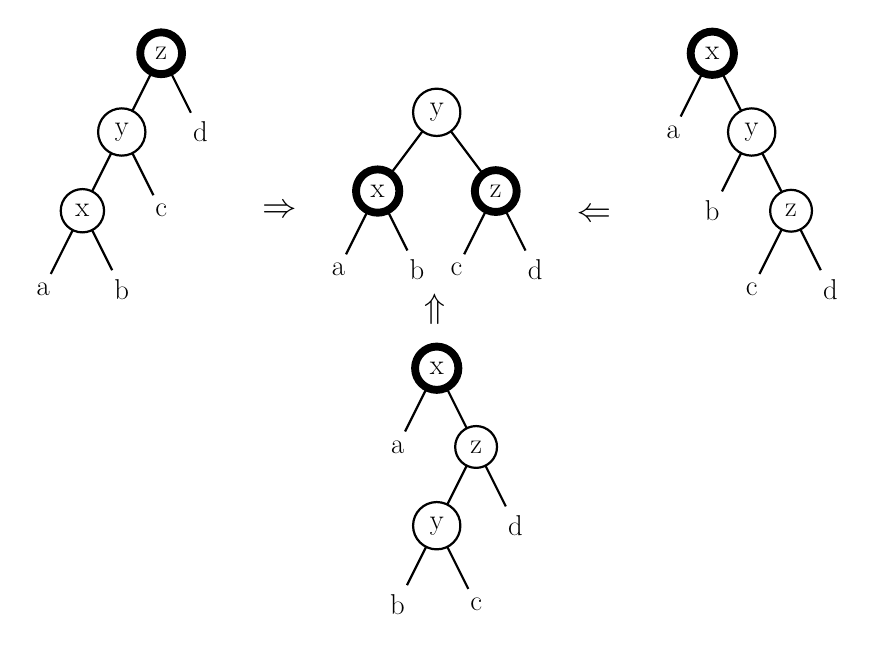
\begin{tikzpicture}[thick,scale=0.5, every node/.style={scale=0.5},level distance=2cm, sibling distance=2cm]
    \tikzstyle{tblack}=[circle, line width=1mm, draw=black]
    \tikzstyle{tred}=[circle, draw=black]
    \def\xstep{7cm}
    \def\ystep{8cm}
    
    \huge
    
%    % legend
%    \begin{scope}[xshift=7cm, yshift=7cm]
%        \def\inse{3.5mm}
%     %   \draw (-1, -2.5) rectangle (5, 1);
%        
%        \node[tblack, inner sep=\inse] at (0,0) {};
%        \node[tred, inner sep=\inse] at (0,-1.6) {};
%        \node[right=1pt] at (1,0) { -- черный};
%        \node[right=1pt] at (1,-1.6) { -- красный};
%    \end{scope}
    
%    \begin{scope}[yshift=\ystep]
%        \node[tblack] {z}
%            child { node[tred] {x}
%                child { node {a} }
%                child { node[tred] {y}
%                    child {node {b}}
%                    child {node {c}}
%                }
%            }
%            child { node {d} };
%    \end{scope}
    
    \begin{scope}[xshift=\xstep]
        \node[tblack] {x}
            child { node {a} }
            child { node[tred] {y}
                child { node {b} }
                child { node[tred] {z}
                    child {node {c}}
                    child {node {d}}
                }
            };
    \end{scope}
    
    \begin{scope}[xshift=-\xstep]
        \node[tblack] {z}
            child { node[tred] {y}
                child { node[tred] {x}
                    child {node {a}}
                    child {node {b}}
                }
                child { node {c} }
            }
            child { node {d} };
    \end{scope}
    
    \begin{scope}[yshift=-\ystep]
        \node[tblack] {x}
            child { node {a} }
            child { node[tred] {z}
                child { node[tred] {y}
                    child {node {b}}
                    child {node {c}}
                }
                child { node {d} }
            };
    \end{scope}
    
    \begin{scope}[yshift=-1.5cm]
        \tikzstyle{level 1}=[sibling distance=3cm]
        \tikzstyle{level 2}=[sibling distance=2cm]
        \node[tred] {y}
            child { node[tblack] {x}
                child { node {a} }
                child { node {b} }
            }
            child { node[tblack] {z}
                child { node {c} }
                child { node {d} }
            };
    \end{scope}
    \Huge
%    \draw (0, 0.5cm) node[rotate=-90] {$\Rightarrow$};
    \draw (0, -6.5cm) node[rotate=90] {$\Rightarrow$};
    \draw (-4cm, -4cm) node[rotate=0] {$\Rightarrow$};
    \draw (4cm, -4cm) node[rotate=180] {$\Rightarrow$};


    
\end{tikzpicture}

%  \caption{Избавление от красных узлов с красными родителями.}
  \label{fig:3.5.2}
\end{figure}
\end{frame}

\begin{frame}[fragile]{}
\begin{hint}
  Даже без дополнительных оптимизаций наша реализация сбалансированных
  двоичных деревьев поиска~--- одна из самых быстрых среди
  имеющихся. С оптимизациями вроде описанных в
  Упражнениях~\ref{ex:2.2} и \ref{ex:3.10} она просто летает!
\end{hint}
\end{frame}


\begin{frame}[fragile]{}
\begin{remark}
  Одна из причин, почему наша реализация выглядит настолько проще, чем
  типичное описание красно-чёрных деревьев 
%  (напр., Глава~14 в книге~\cite{CormenLeisersonRivest1990})
  , состоит в том, что мы
  используем несколько другие преобразования перебалансировки. В
  императивных реализациях обычно наши четыре проблематичных случая
  разбиваются на восемь, в зависимости от цвета узла, соседствующего с
  красной вершиной с красным ребёнком.  Знание цвета этого узла в
  некоторых случаях позволяет совершить меньше присваиваний, а в
  некоторых других завершить балансировку раньше. Однако в
  функциональной среде мы в любом случае копируем все эти вершины, и
  таким образом, не можем ни сократить число присваиваний, ни
  прекратить копирование раньше времени, так что для использования
  более сложных преобразований нет причины.
\end{remark}

\end{frame}


\begin{frame}[fragile]{}
\begin{exercise}\label{ex:3.9}
  Напишите функцию \hsinline{fromOrdList} типа \hsinline{[a] -> Tree a},
  преобразующую отсортированный список без повторений в красно-чёрное
  дерево. Функция должна выполняться за время $O(n)$.
\end{exercise}

\begin{exercise}\label{ex:3.10}
  Приведенная нами функция \hsinline{balance} производит несколько
  ненужных проверок. Например, когда функция \hsinline{ins}
  рекурсивно вызывается для левого ребёнка, не требуется проверять
  красно-красные нарушения на правом ребёнке.
  \begin{enumerate}
    \item Разбейте \hsinline{balance} на две функции
    \hsinline{lbalance} и \hsinline{rbalance}, которые проверяют,
    соответственно, нарушения инварианта в левом и правом
    ребёнке. Замените обращения к \hsinline{balance} внутри
    \hsinline{ins} на вызовы \hsinline{lbalance} либо \hsinline{rbalance}.
    \item Ту же самую логику можно распространить ещё на шаг и убрать
    одну из проверок для внуков. Перепишите \hsinline{ins} так, чтобы
    она никогда не проверяла цвет узлов, не находящихся на пути поиска.
  \end{enumerate}
\end{exercise}
\end{frame}
